\documentclass{article}
\usepackage{styles}

\title{Image Processing\\
    Lab 1}
\author{Kevin Gevers (s25595987) \\ Jeroen Overschie (s2995697)}
\date{\today}

\begin{document}

\maketitle

Note, that all used source code can be found attached next to this report pdf file. Its structure should be self-explanatory; all requested functions are named accordingly and any extra functions are explained in the report. Note that (almost) every function has a corresponding test script, which is named just like its function, but with a suffix '\_test'. Where possible, we followed the terminology from the book \citep{gonzalez2008digital} for variable naming.

\section*{Exercise 1}
In this exercise, \textbf{downsampling}, \textbf{upsampling} and \textbf{zooming} functions are requested. Although we at first implemented them separately, we realized all three are spatial operations that share the same way of geometrically transforming the original image pixel coordinates, just with different scaling factors and/or interpolation method. For example, we can use a scaling constant, say $factor$, to both shrink- (downsampling) using $factor < 1$ and grow an image (upsample) using $factor > 1$. Given these similarities, what then just differs is the \textit{interpolation} method, which can be passed as an argument.

For this reason, we built a generic transformation function, \textsc{IPscaling\_transformation}. This function takes in an image, an (affine) transformation matrix (must be of a certain form) and a parameter controlling which interpolation method to use. Because our requested scaling implementations use this function, we explain this function first.

\subsection*{\textsc{IPscaling\_transformation}}
Like described in the book \citep{gonzalez2008digital} section 2.6 'Geometric Transformations', it is possible to compute new coordinates of some various geometric transformations using just a matrix. Multiplying a coordinate vector by this matrix then produces its new mapped location. Like said in the text, what can be particularly useful of this method is that one can 'stack' various transformations in one matrix, by multiplying various transformation matrices. Even though we do not need this feature in our implementation, we still thought of this mapping step as an elegant way to approach the problem. The scaling transformation matrix $A$ is defined as:

\begin{figure}[ht]
\[A = 
\begin{bmatrix}
cx & 0 & 0\\
0 & cy & 0\\
0 & 0 & 1
\end{bmatrix}
 \]
\end{figure}

With $cx$ and $cy$ the horizontal and vertical scaling factors, respectively. We can now compute the transformed coordinates by multiplying the coordinate vector with the transformation matrix (Eq. 2-45):

\begin{figure}[ht]
\[ 
\begin{bmatrix}
x'\\
y'\\
1
\end{bmatrix}
= A
\begin{bmatrix}
x\\
y\\
1
\end{bmatrix}
 \]
\end{figure}

Even though we can now map from the original image space to the transformed space, it is not trivial how now to determine intensity levels for the unknown pixel values in the transformed space; i.e. interpolation. To make this interpolation process easier later on, we chose to use an \textit{inverse mapping} approach. In inverse mapping, we do not map coordinates from the original space, but rather, we take the transformed coordinates directly and compute the original image position to compute its new intensity value. Given a coordinate in the transformed space, we can obtain its original coordinates using the inverse transformation matrix $A^{-1}$: hence 'inverse' mapping.

\ding{118} For the implementation of \textsc{IPscaling\_transformation}, see Listing~\ref{code:IPscaling_transformation}. We determine the scaled image dimensions by forward mapping the bottom-right coordinate, which is equal to the original image dimensions vector. This indeed returns the scaled image dimensions; but assumes the image only scales, but does not rotate or sheer. This is an assumption we can make, however, because we only perform image scaling indeed.

Now that we have the scaled image dimensions, each output pixel's corresponding original coordinates are computed. Note that we offset the original coordinates by some amount $\sfrac{1}{2}(1 - A^{-1})$ in order to let the original pixels point to the \textbf{centers} of their respective output location.
% [TODO]: explain offset
Given these coordinates we can estimate its new intensity value: using \textbf{interpolation}. We created the \textsc{IPinterpolate} function for this.

\subsection*{\textsc{IPinterpolate}}
The interpolation function has the job of estimating unknown pixel coordinate intensity levels. Having inverse mapped the transformed coordinates, we obtain their position in the original space. Because a scaling operation took place, these probably have decimals: e.g. when growing an 2x2 image to 4x4 size, a pixel in transformed space at $(3, 3)$ would be mapped to $(\sfrac{3}{2}, \sfrac{3}{2})$ like so:

\begin{figure}[ht]
\[ 
\begin{bmatrix}
x \\ y \\ 1
\end{bmatrix} =
\begin{bmatrix}
x' \\ y' \\ 1
\end{bmatrix} A^{-1} =
\begin{bmatrix}
3 \\ 3 \\ 1
\end{bmatrix} A^{-1}=\begin{bmatrix}
3 \\ 3 \\ 1
\end{bmatrix} \begin{bmatrix}
\sfrac{1}{2} & 0 & 0\\
0 & \sfrac{1}{2} & 0\\
0 & 0 & 1
\end{bmatrix}=\begin{bmatrix}\sfrac{3}{2} \\ \sfrac{3}{2} \\ 1
\end{bmatrix}
 \]
\end{figure}

Thus, the challenge lies in estimating values for pixels with unknown intensity values, like $(\sfrac{3}{2}, \sfrac{3}{2})$. We can do this by several means: \textit{Nearest Neighbor interpolation}, \textit{Bilinear interpolation} or \textit{Bicubic interpolation}, among others. Applying no interpolation at all would yield in zero-valued pixels in the output image. Even though the assignment only asked for Nearest Neighbor interpolation and zero-padding, we also implemented Bilinear interpolation out of curiosity.

\ding{118} See Listing~\ref{code:IPinterpolate} for interpolation implementation. Most notably, \textbf{nearest neighbors} works by finding the first available pixel value below the transformed coordinate by using \textsc{round}. Remember that the inverse mapped original coordinates probably have decimals; the rounding operation rounds these coordinates to the nearest pixel in the original space. Note that we are handling images and we can assume we are operating in a \textit{rectilinear grid} with all spacing equal. Using the \textbf{no interpolation} setting just returns a zero-intensity value unless the output pixel can be \textbf{exactly mapped} to an original pixel.

\subsection*{(a)} Now onto the requested functions, which are now easy to implement given the newly available functions. The down-sampling function takes in an image and a scaling factor, $factor$. To down-sample, all we have to do is pass a value $factor < 1$ to \textsc{IPscaling\_transformation}, i.e. to shrink with a factor of 4 we pass $factor = 1/4$.

\ding{118} See implementation: Listing~\ref{code:IPdownsample}. Nearest neighbor interpolation is used and the image is cast to an integer image before saving the result.

\subsection*{(b)} See Figure~\ref{fig:downsampling}. It can be observed that the x4 down-sampled image still looks pretty nice, despite the simple interpolation method used. When down-sampling x15, however, it can be clearly seen that nearest neighbors is not an optimal interpolation method.
\begin{figure}[ht]
    \centering
    \includesvg[width=\textwidth]{Assignment_1/output_plots/cktboard_all_downsamplingFactor=4.svg}
    \caption{Comparison plot of original- and downsampled cktboard image. Middle image shows a factor x4 downsampling and the rightmost image a factor of x15 downsampling.}
    \label{fig:downsampling}
\end{figure}

\subsection*{(c)} Up-sampling is done easily too, using a value of $factor > 1$. Note that it is requested to interpolate by 'introducing zeros'. In our implementation, this corresponds to using \textsc{IPinterpolate} using $interpolation = 'none'$, meaning an output pixel is only assigned an intensity value if its original pixel value could be linearly mapped. This results in unknown pixels having no intensity value, i.e. black pixels. \ding{118} Implementation: Listing~\ref{code:IPupsample}.

\subsection*{(d)} See Figure~\ref{fig:upsampling}. It can be observed that the image is very dark, since a lot of pixels did not get assigned an (interpolated) intensity value.

\begin{figure}[ht]
    \centering
    \includesvg[width=\textwidth]{Assignment_1/output_plots/cktboard_all_upsamplingFactor=4.svg}
    \caption{Comparison plot of original- and upsampled cktboard image.}
    \label{fig:upsampling}
\end{figure}

\subsection*{(e)} Finally, we implement a zooming function. This is upsampling but with interpolation: 'pixel replication' or better, nearest neighbor interpolation. Again we use our generic function, using $factor > 1$ and 'nearest' interpolation. \ding{118} Implementation: Listing~\ref{code:IPzoom}.

\subsection*{(f)} See Figure~\ref{fig:zoom} for a x4 factor zooming of the cktboard image. The zoomed image is 4 times the size, but looks the same, due to pixel replication.
\begin{figure}[ht]
    \centering
    \includesvg[width=\textwidth]{Assignment_1/output_plots/cktboard_all_zoomFactor=4.svg}
    \caption{Comparison plot of original- and zoomed cktboard image.}
    \label{fig:zoom}
\end{figure}

\subsection*{(g)} In this last exercise, we downsample and zoom back in. See Figure~\ref{fig:reconstruction}. Even though the images are back to the same size, we definitely lost some detail. See the bottom image.
\begin{figure}[ht]
    \centering
    \includesvg[width=\textwidth]{Assignment_1/output_plots/cktboard_all_reconstruction=4.svg}
    \includesvg[width=\textwidth]{Assignment_1/output_plots/cktboard_all_zoomed_reconstruction=4.svg}
    \caption{Comparison plot of original- and recontructed cktboard image. The bottom image presents a zoomed-in view of the original and reconstructed image.}
    \label{fig:reconstruction}
\end{figure}

\subsection*{Bilinear interpolation extra}
Out of curiosity, we compared our nearest neighbor interpolation with \textbf{Bilinear interpolation}. It is a bit more complicated, but still relatively easy. It uses the 4 nearest neighbors to compute a weighting each pixel has on the estimated intensity value. It can be expressed as $v(x, y) = ax + by + cxy + d$. Since we are estimating intermediate pixel values, we get a much smoother output image. See Figure~\ref{fig:bilinear}. It can be observed that our method performs very similarly using both interpolation methods to Matlab's built-in function.

\begin{figure}[ht]
    \centering
    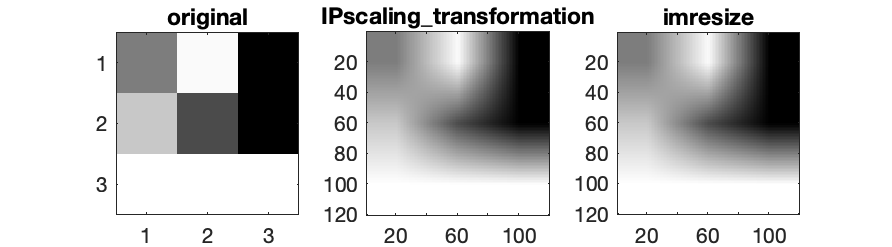
\includegraphics[width=\textwidth]{Assignment_1/output_plots/matrix_all_bilinear_factor=40.png}
    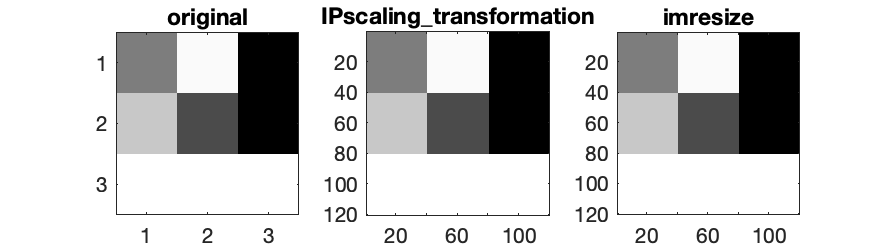
\includegraphics[width=\textwidth]{Assignment_1/output_plots/matrix_all_nearest_factor=40.png}
    \includesvg[width=\textwidth]{Assignment_1/output_plots/asdfasdf=4.svg}
    \caption{Comparison plot of original- and reconstructed cktboard image. The bottom image presents a zoomed-in view of the original and reconstructed image.}
    \label{fig:bilinear}
\end{figure}

\section*{Exercise 2}
\subsection*{a} \ding{118} Implementation: Listing~\ref{code:IPhistogram}.

\subsection*{b} \ding{118} Implementation: Listing~\ref{code:IPhisteq}.

\subsection*{c}


\section*{Exercise 3}
\subsection*{a}

\subsection*{b}

\subsection*{c}

\bibliographystyle{plain}
\bibliography{Assignment_1}

\appendix
\section{Code}
\subsection{Exercise 1}
\lstinputlisting[caption={IPscaling\_transformation.m: perform geometric transformations of \\the \textit{scaling} kind, given an affine transformation matrix or a scaling constant.}, label={code:IPscaling_transformation}]{Assignment_1/IPscaling_transformation.m}
\lstinputlisting[caption={IPinterpolate.m: interpolate an unknown pixel intensity value using\\ one of the supported methods.}, label={code:IPinterpolate}]{Assignment_1/IPinterpolate.m}
\subsubsection{Exercise 1 (a)}
\lstinputlisting[caption={IPdownsample.m: downsample images using \textsc{IPscaling\_transformation}.}, label={code:IPdownsample}]{Assignment_1/IPdownsample.m}
\subsubsection{Exercise 1 (c)}
\lstinputlisting[caption={IPupsample.m: upsample images using \textsc{IPscaling\_transformation}.}, label={code:IPupsample}]{Assignment_1/IPupsample.m}
\subsubsection{Exercise 1 (e)}
\lstinputlisting[caption={IPzoom.m: zoom images using \textsc{IPscaling\_transformation}.}, label={code:IPzoom}]{Assignment_1/IPzoom.m}
\subsection{Exercise 2}
\subsubsection{Exercise 2 (a)}
\lstinputlisting[caption={IPhistogram.m: construct an image's histogram.}, label={code:IPhistogram}]{Assignment_1/IPhistogram.m}
\subsubsection{Exercise 2 (b)}
\lstinputlisting[caption={IPhisteq.m: histogram equalization.}, label={code:IPhisteq}]{Assignment_1/IPhisteq.m}

\end{document}
